\documentclass[10pt,journal]{IEEEtran}

\usepackage{amsmath,amssymb,bm}
\usepackage{graphicx}
\usepackage{booktabs}
\usepackage[table]{xcolor}
\usepackage{caption}
\usepackage{microtype}
\usepackage[hidelinks]{hyperref}

\newcommand{\blur}{\star}
\newcommand{\Lam}{\Lambda}
\newcommand{\kunif}{\kappa}
\newcommand{\E}{\mathbb{E}}

\begin{document}

\title{Quantifying Blur Preference in Diffusion Priors: Spectral Scaling and Implications
for Blind Image Deconvolution}

\author{Bin~Nong~and~Weihong~Fu%
\thanks{B.~Nong is with the Tianfu College of Southwestern University of Finance
and Economics, Mianyang, China, and is the corresponding author
(e-mail: nongbin@tfswufe.edu.cn).}%
\thanks{W.~Fu is with the School of Telecommunications Engineering, Xidian University,
Xi'an, Shaanxi, China.}}

% Running heads are left to the publisher: the IEEEtran sample \markboth placeholder
% ("Journal of \LaTeX\ Class Files, Vol. XX, No. XX") was removed before submission.

\maketitle

\begin{abstract}
We quantify the previously reported preference of diffusion priors for blurred images using the
paired log-ratio $\Lam(t,u)=\log p_t(h\blur x)-\log p_t(x)$, where $u$ is retained spectral
power. For an EDM/FFHQ-64 prior evaluated on its generated samples, a single-image scan gives
$3.2\times10^4$ nats at $t=0.002$. On 32 selected real BSDS300 test images, all 256 low-noise
image--kernel pairs are positive ($32/32$ image-level successes; exact 95\% interval
$[0.8911,1]$); $120/128$ pairs are positive at $t=0.20$. Seven smooth profiles admit
$\Lam\approx\mathcal M(\mathrm{shape})u^{b_\infty}\exp((A/q)u^q)$, with
$b(u)=\mathrm d\log\Lam/\mathrm d\log u\approx b_\infty+Au^q$, tested on four unseen shape
classes plus a control. The form fits through $t=0.05$ in the tested range and degrades at
$t=0.16$; its parameters and shape factor are not universal. A full-Fourier, full-RGB
spectrum-matched Gaussian underestimates the low-noise preference by $12.57\times$ in one
representative case. Continuous VP-ODE surrogate pilots on two ADM checkpoints show model- and
noise-level dependence, but do not establish equality with the original discrete-model densities.
For blind deconvolution, we distinguish a smoothed-prior MAP surrogate from the exact clean-image
posterior and give an algebraic no-blur objective gap. Because a diffusion denoiser is not
generally the proximal map of that potential, our Douglas--Rachford plug-and-play experiments
are feasible-point grid studies, not certified profile-MAP minimisation. Their grid selections
over-blur in $79/80$ Gaussian configurations but frequently under-blur in multi-kernel and real
BSDS pilots. A direct score-gradient pilot instead under-blurs in all eight four-probe-mean
profiles, demonstrating that the PnP direction does not transfer automatically to the declared
objective; this is not a global-optimality or restoration-quality result. A spectral correction
does not consistently improve kernel error. Clean-pair preference must not be interpreted as
noisy-posterior preference or as a demonstrated restoration improvement.
\end{abstract}

\begin{IEEEkeywords}
Blind deconvolution, diffusion models, score-based generative models, inverse problems,
image restoration, maximum a posteriori estimation, blur estimation.
\end{IEEEkeywords}

\section{Introduction}
\label{sec:intro}

Blind image deconvolution asks for a sharp image and an unknown blur operator from a single
degraded observation. Diffusion and score-based priors
\cite{ho2020ddpm,song2021score,nichol2021improved,song2020improved} are widely used for
inverse problems. A substantial family of blind methods alternates
between an image update and an operator update, each conditioned on the other
\cite{chung2023bdm,murata2023gibbsddrm,laroche2024fastdiffusionem,bai2026ladibi}, or
marginalises the operator out of a joint diffusion process
\cite{song2023resample,wang2022ddsm,kawar2022ddrm}.

Such objectives need not treat the prior as a neutral referee: a systematic density preference
between image--blur pairs can also influence operator estimation. The prior must account for
image content removed by blur, rather than implicitly favouring a particular operator strength.
We measure this preference directly rather than assuming its sign or its effect on an estimator.

The object of this paper is the
\emph{blur preference}
\begin{equation}
  \Lam(t,u) \;=\; \log p_t(h\blur x) \;-\; \log p_t(x),
  \label{eq:lam}
\end{equation}
where $t$ is the diffusion noise level, $h$ a blur operator with power spectrum
$\{|\hat h(f)|^2\}$, and $u$ is its mean retained power on the implemented non-redundant
rFFT grid (Section~\ref{sec:measurement} distinguishes this from the full-grid average).
Equation~\eqref{eq:lam} is a \emph{paired} log-ratio: both terms are evaluated
on the same image with the same estimator, so no reference posterior, no baseline, and no
calibration constant enters. It is therefore a directly measurable property of the prior, and it
is what this paper measures.

Our central empirical finding is that $\Lam$ is positive and large at the low-noise end for a
mild blur (Section~\ref{sec:phen}), and is governed largely by $u$ in the tested regime
(Section~\ref{sec:law}). Section~\ref{sec:mech} compares it with three stationary
Gaussian/spectral references; these are not equivalent to a general local second-order Taylor
approximation. Section~\ref{sec:map} then gives a transparent decomposition of a no-blur MAP
objective gap. Its algebraic exactness does not remove the need to establish convergence of the
numerical inner optimiser, and our finite experiments do not decide a universally quantified
lemma. Section~\ref{sec:overblur} separately documents PnP-grid over-blurring on a specified
Gaussian-kernel grid without equating that grid selection with a profile-MAP solution.

\paragraph*{Contributions}
\begin{enumerate}
  \item A paired measurement with an exact terminal-density calculation and bound, a terminal
        audit over 960 image--kernel pairs, separate 32-repeat checks, and a shared-probe
        full-curve audit of trace and integration-tolerance effects on the fitted exponent
        (Sections~\ref{sec:measurement} and~\ref{sec:law}).
  \item A controlled experiment separating total attenuation from profile shape, yielding
        $\Lam\approx \mathcal M(\mathrm{shape})u^{b_\infty}\exp((A/q)u^q)$ and hence
        $b(u)=\mathrm d\log\Lam/\mathrm d\log u\approx b_\infty+Au^q$, with
        $b_\infty\approx-0.73$, $A\approx-7.2$, and $q\approx3.4$ at $t=0.002$
        (Section~\ref{sec:law}).
  \item A quantified delimitation of stationary Gaussian and operator-spectral approximations,
        plus a directional local-quadratic test of the ODE potential; no full-Hessian or
        all-local-methods claim (Section~\ref{sec:mech}).
  \item A fully defined algebraic no-blur objective gap, PnP-grid studies, and a direct
        score-gradient pilot with endpoint trace replication. We distinguish the smoothed-prior
        surrogate from the original clean-image posterior, and a denoiser-based fixed point
        from a proximal or profile-MAP solution (Sections~\ref{sec:map} and~\ref{sec:overblur}).
  \item Full disclosure of a half-pixel kernel bug that corrupted thirteen scripts, together
        with corrected numbers and an independent cross-check (Section~\ref{sec:bug}).
\end{enumerate}

\paragraph*{Scope}
This is an empirical study, not a theorem about all diffusion priors or all second-order
methods. The main measurements use EDM/FFHQ at $64\times64$, with EDM/AFHQv2 as a limited
second-checkpoint comparison. Their main image pools are model-generated; separate experiments
use 32 real BSDS300 test images for density measurements and eight for PnP profiles. We therefore
do not claim cross-architecture, cross-resolution, real-FFHQ, general natural-image
universality, exact profile-MAP convergence, or an improved restoration algorithm.

\section{Related work}
\label{sec:relwork}

\paragraph*{Blind deconvolution with diffusion priors}
The line this paper belongs to attacks blind inverse problems by giving the unknown operator its
own generative or sampling process. Chung et al.\ diffuse the operator and the image jointly in
parallel \cite{chung2023bdm}; GibbsDDRM partially collapses the same problem into a Gibbs
sampler over DDRM \cite{murata2023gibbsddrm}; Fast Diffusion EM treats the operator as a latent
variable in an EM loop for deconvolution \cite{laroche2024fastdiffusionem}; and LADiBI inverts
with a latent diffusion prior \cite{bai2026ladibi}. A second family marginalises the operator
out of a null-space or consistency-constrained model
\cite{song2023resample,wang2022ddsm,kawar2022ddrm}. The non-blind ancestors of the same idea
approximate the posterior directly \cite{chung2022dps} or learn to invert a latent prior under a
task prompt \cite{chung2023prompttuning}. Plug-and-play formulations
\cite{venkatakrishnan2013pnp,sreehari2016pnp} and their diffusion instantiations
\cite{zhu2023dpnp} are the non-blind ancestor of the same idea. Surveys of the area
\cite{daras2024survey,luo2025taming,zhang2025survey} are the standard entry points. The
classical formulation the field grew out of---alternating image and kernel updates under a
sparse or natural-image prior, with its characteristic failure modes diagnosed empirically
\cite{levin2009understanding,levin2011understanding} and its marginal-likelihood variant
\cite{levin2011efficient}---predates learned priors entirely; convex relaxations
\cite{ahmed2014blind} and learned kernel estimators \cite{xu2018motion,ren2020neural} and
restoration networks \cite{zamir2022restormer,chen2022nafnet} are the non-diffusion deep
baselines. The blurry preference itself is older than learned priors: Perrone and Favaro analyse
the log probability of natural against blurred images under classical logarithmic and Cauchy-type
priors and build a blind deconvolution method on it \cite{perrone2016logarithmic}, which is the
sparse-prior origin of the ``blurry trap'' that \cite{nguyen2025morsebott} refers to. The same
group's later diffusion-prior work \cite{chihaoui2025diip} is a zero-shot restoration
\emph{method}---blind, degradation-agnostic, driven by early stopping---rather than a measurement
of the gap; the two together bracket the prior generations across which the effect persists.
Bayesian treatments of plug-and-play and half-quadratic priors
\cite{laumont2022bayesian,kemajou2024marginal} are the closest non-diffusion relatives of the
profile-MAP analysis in Section~\ref{sec:overblur} (see also \cite{murphy2000profile}).

\paragraph*{What is already in the literature, stated precisely}
The phenomenon and several related theoretical results are established. We distinguish four
strands.

(i) \emph{The phenomenon, measured qualitatively.} Nguyen et al.\ evaluate the potential
$q(h_\theta\blur x)$ as the blur scale $\theta$ grows, over four one-dimensional blur families
and a hundred images, and report it decreasing strictly on FFHQ-256, ImageNet-64, FFHQ-64 and
AFHQ-64, concluding $p_{\boldsymbol{x}}(h_\theta\blur x)>p_{\boldsymbol{x}}(x)$
\cite{nguyen2025morsebott}\S4.1. They also run the control we would have wanted: a diffusion
model trained on binarized MNIST, where the tendency \emph{reverses}, which they read as
evidence that the preference is a property of natural-image statistics rather than of the network
architecture. Their images are drawn from the model's training set.

(ii) \emph{A sufficient condition for global MAP failure.} The same paper's Lemma~12 states that
if $q(h\blur x)\le q(x)$ for all $x$ and all $h$ in the kernel set, then the global minimiser
contains a degenerate no-blur pair; their \S4.1 is offered as numerical verification that the
condition holds. The related-lineage paper \cite{debarnot2023blind} develops the blind-setting
analysis further.

(iii) \emph{Why it should be expected.} Natural images concentrate near a low-dimensional
manifold, so off-manifold and degraded images have low density; this has counterparts in the
manifold-hypothesis convergence analysis of diffusion models \cite{debortoli2022manifold} and in
the result that score-based models detect manifolds \cite{pidstrigach2022manifolds}.

(iv) \emph{High density coincides with blur.} Karczewski et al.\
\cite{karczewski2025cartoonists} construct a sampler that provably yields higher-likelihood
samples and find the resulting high-density regions are cartoon-like drawings or blurry images
depending on the noise level---an effect present even in datasets containing no such images. The
base paper explicitly cites them as an independent confirmation of the preference for blur, and
notes that the two works were produced independently at roughly the same time.

\paragraph*{What the present study adds}
Prior work already reports both blurry high-density regions and MAP failure; those discoveries
are not ours. Our narrower contribution is a paired normalised log-density difference in nats,
on the common axis $u$, with its noise-level dependence and an explicit numerical-uncertainty
discussion. In the tested regime we further fit
$\mathcal M(\mathrm{shape})u^{b_\infty}\exp((A/q)u^q)$, validate it on unseen profile shapes, and quantify
where three stationary Gaussian/spectral references agree or diverge. For blind deconvolution we provide a
fully expanded algebraic bookkeeping identity and a controlled empirical over-blur study. These
additions complement, rather than supersede, the qualitative and theoretical results of
\cite{nguyen2025morsebott,karczewski2025cartoonists}.

We therefore claim a \emph{quantitative measurement and empirical scaling law}, not discovery
of the effect. Our literature search covered OpenAlex/arXiv keyword queries, citation and
similarity expansion from \cite{nguyen2025morsebott,karczewski2025cartoonists,karras2022edm},
and ordinary web search. The inspected work on high-density sampling steers generation toward
such regions rather than measuring a paired image--degradation contrast; we did not find the
present $\Lam(t,u)$ measurement in those sources. This is a scoped literature search, not a
systematic-review guarantee of priority.

\paragraph*{Two adjacent literatures that are \emph{not} the same thing}
Spectral bias in diffusion models has recently been studied analytically and empirically
\cite{wang2025spectralbias,urfin2026spectralbias}, but in the sense of \emph{training}
dynamics---which frequencies a model learns first. Our claim is about the prior at inference:
a fixed trained model's preference between two images it did not generate. Separately,
``blurring diffusion models'' \cite{hoogeboom2023blurring} places blur inside the generative
forward process, which changes the model rather than probing it. Neither line measures
$\Lambda$.

\paragraph*{Positioning relative to the Morse--Bott framework}
Nguyen, Pauwels and Weiss \cite{nguyen2025morsebott} give local recovery guarantees and exhibit
the failure of the MAP estimate for blind inverse problems. Their Lemma~12 uses the universally
quantified hypothesis $q(h\blur x)\le q(x)$ for every image and every kernel in a specified set.
For one fixed pair, this inequality is equivalent by definition to $\Lam_{\rm clean}\ge0$. That
sample-wise equivalence neither proves nor disproves the universal hypothesis. Accordingly,
Section~\ref{sec:map} reports only a 15-configuration sign-consistency check and does not claim
to decide the lemma's validity boundary.

\section{Measurement}
\label{sec:measurement}

\subsection{The quantity}

Let $q_t(z)=-\log p_t(z)$ denote the prior potential; data fidelity is denoted separately by
$D$ below. Let $x^\blur=h\blur x$. The blur preference of~\eqref{eq:lam} compares the density
of the blurred and sharp images \emph{at the same noise level} $t$, where $p_t$ is the marginal
of the EDM forward process:
$p_t(x)=\int p_{\rm data}(x_0)\,\mathcal N(x;x_0,t^2I)\,\mathrm dx_0$.
This is a normalised density, not a score or an unnormalised energy. Both terms use the same
solver and integration grid; stochastic trace error is treated as estimator variability rather
than assumed to cancel. Pairing removes image-independent additive integration constants, but
not the image-dependent terminal term.

We next derive that term without identifying an operator average with an image energy ratio.
At $\sigma_{\max}=80$, the Gaussian terminal contribution to the log-ratio is
\begin{equation}
  T(x,h)=\frac{\|x\|^2-\|h\blur x\|^2}{2\sigma_{\max}^2}
  =\frac{\sum_f(1-|\hat h(f)|^2)|\hat x(f)|^2}
         {2\sigma_{\max}^2},
  \label{eq:terminal}
\end{equation}
where the last equality is Parseval's identity with a consistent FFT normalisation. If
$r_{x,h}=\|h\blur x\|^2/\|x\|^2$, then $T=(1-r_{x,h})\|x\|^2/(2\sigma_{\max}^2)$; in general
$r_{x,h}\ne u$. For every contractive operator used here, $0\le|\hat h(f)|^2\le1$, so
\begin{equation}
  0\le T(x,h)\le \frac{\|x\|^2}{2\sigma_{\max}^2}
  \le\frac{N}{2\sigma_{\max}^2}=0.96\ \text{nats},
  \label{eq:terminal_bound}
\end{equation}
because $N=12288$ and pixels lie in $[-1,1]$. The ODE density evaluation already includes this
terminal contribution; we do not apply an additional $u$-based correction. Thus terminal
normalisation can account for at most $0.96$ nats of a measured $\Lam$, independently of the
non-flat image spectrum.

We parameterise operators by their power spectrum rather than by a kernel parameter, because
kernel parameters are not comparable across families. Let $g_2(f)=|\hat h(f)|^2$ and let
$\mathcal R$ denote the implemented $64\times33$ rFFT grid. The empirical coordinate is
\begin{equation}
  \kunif \;=\; \big\langle 1-g_2\big\rangle_{\mathcal R}, \qquad
  u \;=\; 1-\kunif \;=\; \big\langle g_2\big\rangle_{\mathcal R}.
  \label{eq:kunif}
\end{equation}
It is an unweighted mean on that grid, not automatically the full-FFT average. For real images,
the conjugate multiplicity is $c_f=1$ in rFFT columns 0 and 32 and $c_f=2$ otherwise; full-FFT
Parseval sums therefore use $\sum_{f\in\mathcal R}c_f$. The corresponding full-grid retained
power is $u_{\rm full}=\sum_{f\in\mathcal R}c_f g_2(f)/\sum_{f\in\mathcal R}c_f$, which is used
for exact Gaussian expectations below. Across the eight raw reference kernels, $u-u_{\rm full}$
is $0.0015$--$0.0085$; these are different conventions, not interchangeable identities. We
retain $u$ for the measured curves and fitted law rather than silently changing their coordinates.
A stronger blur has smaller $u$ along each fixed-shape path; $u=1$ is the identity and $u=0$
annihilates everything. All curves below are plotted against this declared empirical coordinate.
Source: \texttt{results/fullfft\_reference\_audit.json}.

\subsection{Image-pool provenance}
\label{sec:pools}

The main FFHQ-labelled input is a 256-image pool generated by the released EDM/FFHQ checkpoint
using \texttt{repro/make\_pool.py}; it is not a real FFHQ dataset split. The main scaling
experiments use samples 0--119, the two Gaussian PnP-profile pools use the disjoint index sets
0--19 and 20--39, and the multi-kernel pilot uses 40--47. Samples 128--255 calibrate the spectral
correction, and sample 255 is used for the single-image numerical checks. The analogous AFHQv2
pool is also model-generated. These pools are suitable for probing properties of the learned
prior, but they do not establish external validity on real images. Earlier internal labels
``real pool'' and ``held-out'' were incorrect; they are not used as evidence here.

\subsection{Numerical evaluation}

Log-densities come from the probability-flow ODE of the EDM parameterisation
\cite{karras2022edm}, integrated with the same solver and step count for both
images of a pair, with the divergence term estimated by a Skilling--Hutchinson trace estimator
\cite{skilling1989eigenvalues,hutchinson1990stochastic}. The model is the released \texttt{edm-ffhq-64x64-uncond-vp}
checkpoint; all experiments are at $64\times64$ RGB ($N=12288$ scalar samples), which is the
resolution at which FFHQ weights are published.

That the returned number is a normalised log-density, and not a divergence integral up to an
unknown offset, was established before any measurement was taken. On an exactly Gaussian prior
the probability-flow ODE has the analytic solution
$-\log p_t(x)=\|x\|^2/(2(s^2+t^2))+(N/2)\log 2\pi(s^2+t^2)$, and the numerical integration
reproduces it, with the Tweedie identity and the ODE drift term both agreeing to $10^{-9}$. We
rely on that check only for the absolute scale: $\Lam$ is a difference and would survive an
unknown additive offset, which is why the pairing in Section~\ref{sec:measurement} is what
makes the quantity measurable at all.

Two implementation details matter for reproducibility. First, every physical Gaussian kernel
used in this paper is taken from the library implementation rather than hand-written, for the
reason given in Section~\ref{sec:bug}. Second, $t$ is kept at or above the $0.002$ training
noise floor. The released preconditioner has $\sigma_{\min}=0$, so its bounds alone do not
guard against evaluating the model below that floor.

\subsection{Repeatability and statistical uncertainty}
\label{sec:uncertainty}

\paragraph*{Terminal-term audit across images and kernels.}
We evaluated~\eqref{eq:terminal} directly on 120 images and all eight raw reference kernels
(960 image--kernel pairs). The exact terminal term ranges from $0.0066$ to $0.2436$ nats,
with per-kernel means $0.0167$--$0.0904$ nats. The retired $u$-based approximation has errors
up to $0.5898$ nats. These measurements both confirm the bound in~\eqref{eq:terminal_bound}
and quantify why the exact image spectrum, rather than $u$, is required. Source:
\texttt{results/review\_numeric.json}.

\paragraph*{Hutchinson and across-image variability.}
The original four repeats gave $\mathrm{sd}(\Lam)=388$ nats at one low-noise configuration and
are retained in Fig.~\ref{fig:phen} only as a pilot scale. A new set of 32 independent pairs at
the same image/operator gives mean $\Lam=31851.9$, SD $306.5$, and mean SE $54.2$ nats at
$t=0.002$. At $t=0.20$, 32 pairs give $195.3$ nats, SD $58.0$, and mean SE $10.3$ nats
(normal 95\% mean interval $[175.2,215.4]$). Thus the high-noise preference is resolved above
zero, while its magnitude remains estimator-dependent. Across-image variability is reported
separately by image standard deviations, standard errors, and cluster bootstraps.

\paragraph*{Adaptive ODE integration error.}
With one fixed Hutchinson vector shared across solver settings, we scanned RK45 tolerances
$10^{-3}$--$10^{-6}$ and compared against DOP853 at $10^{-6}$. The default RK45
($10^{-5}$) differs from that reference by only $-0.148$ nats at $t=0.002$ and $+0.078$ nats
at $t=0.20$. Coarse RK45 at $10^{-3}$ differs by $62.6$ and $1.91$ nats, respectively, showing
that the tolerance rather than the pairing accounts for the integration discrepancy. This is an
adaptive-solver/tolerance check, not a fixed-step scan. Source:
\texttt{results/review\_numeric.json}.

\section{Measured blur preference across operators and noise levels}
\label{sec:phen}

Nguyen et al.\ previously established the qualitative sign across four one-dimensional blur
families and several datasets \cite{nguyen2025morsebott}\S4.1. Our contribution here is the
paired magnitude on a common axis, its cross-image distribution, and its noise-level
dependence, with numerical uncertainty stated separately.

Figure~\ref{fig:phen} shows $\Lam$ against $u$ for eight physically distinct blur kernels---
Gaussian at two widths, defocus at two radii, an Airy disc, motion blur at two lengths, and an
ideal low-pass---measured on the 120 model-generated images of Section~\ref{sec:pools} at
$t=0.002$. The horizontal axis is
$u=\langle|\hat h|^2\rangle$, rather than an incomparable per-family parameter $\theta$. The
figure reports image-to-image variation; the four-repeat Hutchinson estimate from
Section~\ref{sec:uncertainty} is shown only as a separate pilot repeatability scale.

\begin{figure*}[t]
  \centering
  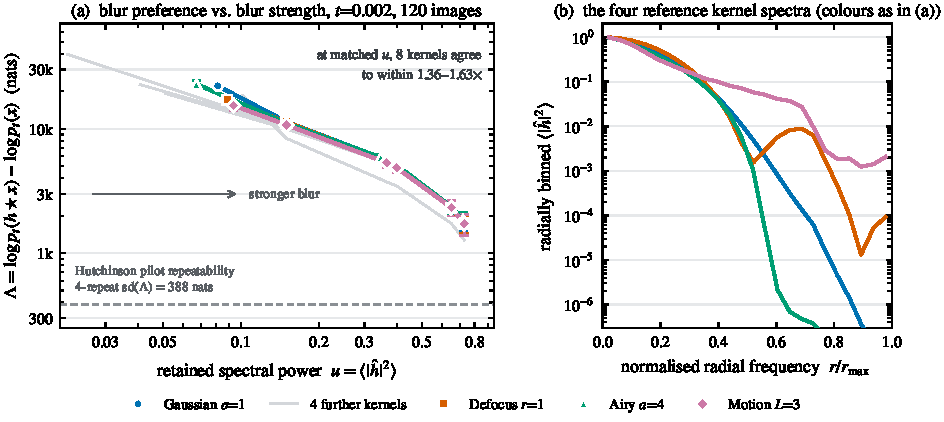
\includegraphics[width=\textwidth]{fig_phenomenon.pdf}
  \caption{%
    \textbf{(a)} Blur preference $\Lam$ against retained spectral power $u$ at $t=0.002$,
    mean~$\pm$~s.d.\ over 120 images, for four representative kernels (colour, markers with
    error bars) and four further kernels (grey). The dashed line marks the four-repeat
    Hutchinson pilot standard deviation, $388$ nats, not a universal error bound.
    \textbf{(b)} Radially binned power spectra $\langle|\hat h|^2\rangle$ of the four coloured
    kernels. At matched $u$ the eight kernels agree to within $1.36$--$1.63\times$.}
  \label{fig:phen}
\end{figure*}

The plotted means are positive and decrease as $u$ increases; the eight curves nearly coincide.
At six matched values of $u$, the spread across the kernels that reach that $u$---eight at four
of them, seven and five at the other two---is $1.36$--$1.63\times$ (median $1.49\times$). This
near-coincidence occurs despite the visibly different Gaussian, defocus, Airy, and motion
spectra in panel~(b). It is an empirical collapse over these operators, not a consequence that
any arbitrary spectral functional must share.

Table~\ref{tab:lamt} is deliberately a single-image scan, not a cross-image average. Its point
estimates decrease from $3.2\times10^{4}$ nats at $t=0.002$ to $1.6\times10^{2}$ nats at
$t=0.20$. The final single draw is below the old $388$-nat pilot scale, but the independent
32-repeat measurement reported above resolves its mean as $195.3\pm10.3$ nats (SE). The table
therefore shows a noise-level trajectory, not a per-row confidence statement. A full-RGB,
full-Fourier spectrum-matched Gaussian is $12.57\times$ below the measured preference at
$t=0.002$, but exceeds its point estimate at $t=0.10$ and $0.20$; this is not a uniform failure
across noise levels.

\begin{table}[t]
  \centering
  \caption{Blur preference $\Lam$ against diffusion noise level $t$ for one EDM/FFHQ-generated
  image and Gaussian $\sigma=1.5$, using the corrected kernel. These are individual point
  estimates, not per-row means. Independent 32-repeat measurements at $t=0.002$ and $0.20$ give
  $31851.9\pm54.2$ and $195.3\pm10.3$ nats (mean $\pm$ SE), respectively. $\Lam_{\rm Gauss}$
  uses conjugate-complete Fourier weights and all RGB channels, calibration-pool radial variances
  plus $t^2$, and the sharp image's periodogram. Sources: \texttt{results/tdep\_kfix.json},
  \texttt{results/review\_numeric.json}, and \texttt{results/fullfft\_reference\_audit.json}.}
  \label{tab:lamt}
  \begin{tabular}{crrr}
    \toprule
    $t$ & $\Lam$ & $\Lam_{\rm Gauss}$ & $\Lam/\Lam_{\rm Gauss}$ \\
    \midrule
    0.002 & 31966 & 2542.6 & 12.57 \\
    0.005 & 26560 & 2528.7 & 10.50 \\
    0.01  & 21147 & 2482.8 &  8.52 \\
    0.02  & 12272 & 2338.9 &  5.25 \\
    0.05  &  3425 & 1859.9 &  1.84 \\
    0.10  &   917 & 1292.5 &  0.71 \\
    0.20  &   162 &  725.0 &  0.22 \\
    \bottomrule
  \end{tabular}
\end{table}

\subsection{What is \emph{not} claimed}
These measurements concern clean image pairs. After observation noise is added, the blurred
observation has lower estimated density than the sharp observation in $85/100$ pairs from twenty
images and five noise levels (whole-image cluster-bootstrap 95\% interval $[0.79,0.91]$ for the
proportion), and in $77/80$ pairs with $\sigma_n\ge0.02$. Thus the clean-image preference must
not be interpreted as the sign of the full noisy posterior. Nor does it by itself imply that an
operator argmin moves; Section~\ref{sec:overblur} tests that separate claim empirically.

\subsection{External validation on real natural images}
\label{sec:real}

We repeated the measurement on the first 32 sorted images of the official BSDS300 test split
\cite{martin2001bsds}. These are real natural images, not model samples or an FFHQ dataset split.
Images are converted to RGB, resized with Lanczos on the short side, centre-cropped to
$64\times64$, and mapped to $[-1,1]$. At $t=0.002$, every one of the 256 image--kernel pairs
has $\Lam>0$; the whole-image cluster 95\% interval for the mean is $[24926,26983]$ nats.
Because all eight kernels are positive on each of the 32 images, the image-level success count
is $32/32$, whose two-sided 95\% Clopper--Pearson interval is $[0.8911,1]$; zero observed
failures do not imply certain population positivity. At $t=0.20$, $120/128$ raw pairs are
positive and the cluster-mean interval is $[938.9,1493.5]$ nats. All four tested kernels are
simultaneously positive on $27/32$ images, giving the image-level Clopper--Pearson interval
$[0.6721,0.9472]$. The raw pair counts retain within-image dependence and are not treated as
256 or 128 independent Bernoulli trials. This establishes external validity on the selected real
natural images, not a universal sign or a real-FFHQ validation. Table~\ref{tab:real_bsds} gives
all configurations. Sources: \texttt{results/real\_bsds\_edm.json} and
\texttt{repro/analyze\_review2.py}.

\begin{table}[t]
  \centering
  \caption{Real-BSDS blur preference $\Lam$ (nats), mean and positive count over 32 images per
  cell. The test uses the same EDM/FFHQ checkpoint and numerical protocol as the generated pools.
  A dash denotes a configuration not measured.}
  \label{tab:real_bsds}
  \small
  \setlength{\tabcolsep}{3pt}
  \begin{tabular}{lcccc}
    \toprule
    Kernel & \multicolumn{2}{c}{$t=0.002$} & \multicolumn{2}{c}{$t=0.20$}\\
    \cmidrule(lr){2-3}\cmidrule(lr){4-5}
    & Mean & Positive & Mean & Positive\\
    \midrule
    Gaussian 1 & 24515.2 & 32/32 & 1095.5 & 30/32\\
    Gaussian 2 & 44491.9 & 32/32 & 1420.6 & 31/32\\
    Defocus 1 & 19760.6 & 32/32 & 1098.7 & 28/32\\
    Defocus 2 & 25724.0 & 32/32 & --- & ---\\
    Airy 4 & 26032.5 & 32/32 & --- & ---\\
    Motion 3 & 18511.0 & 32/32 & 1250.7 & 31/32\\
    Motion 7 & 22773.3 & 32/32 & --- & ---\\
    Ideal low-pass & 25890.9 & 32/32 & --- & ---\\
    \bottomrule
  \end{tabular}
\end{table}

\subsection{Non-EDM and native-resolution pilots}
\label{sec:adm}

We next test two OpenAI ADM checkpoints on real BSDS images: the unconditional
improved-diffusion ImageNet-64 model \cite{nichol2021improved} and the native $128\times128$
guided-diffusion ImageNet model \cite{dhariwal2021diffusion}. The latter is evaluated as a
fixed-label (0) conditional prior without classifier guidance; it is not an unconditional prior.
For these discrete epsilon-prediction models we construct a continuous VP-ODE surrogate:
log-linearly interpolate the cumulative-alpha schedule, evaluate the network with its continuous
sinusoidal timestep embedding, and integrate the probability-flow drift with a Gaussian terminal
state. This is not a discrete DDPM variational bound. The adapter recovers an analytic Gaussian
potential to $1.88\times10^{-4}$ nats. The physical noise coordinate is $\sigma$; the 64/128
checkpoints are restricted to $\sigma\ge0.005/0.05$ here because of their schedules. Each pair
shares one Rademacher trace vector. At one $64\times64$ configuration, default RK45 differs from
DOP853 at $10^{-6}$ by $47.5$ nats, about $0.19\%$ of that preference; this is a single-point check.
For the native-128 Gaussian-1 example, DOP853 gives $41323.3$ and $-14033.2$ nats at
$\sigma=0.05$ and $0.20$, respectively. Default-minus-DOP853 differences are $273.8$ and $-51.0$
nats and preserve both signs, so the reversal is not an RK45 artifact in this example.

Table~\ref{tab:adm} shows that the unconditional non-EDM $64\times64$ model has positive preference
in all 96 tested pairs across three noise levels. The native-128 conditional model instead reverses
sign between $\sigma=0.05$ and $0.20$, with $16/16$ positive and $0/16$ positive, respectively.
Architecture, training data, conditioning, and resolution differ jointly in this comparison;
it is not a controlled resolution-only experiment. It establishes model/noise dependence only
for these constructed surrogate priors. The analytic Gaussian guard validates the integrator,
not equality between the continuous surrogate density and the original discrete-DDPM model.
Sources: \texttt{results/adm64\_analysis.json}, \texttt{results/adm128\_analysis.json}, and
\texttt{results/adm128\_numeric.json}.

\begin{table}[t]
  \centering
  \caption{ADM pilots on real BSDS images using the constructed continuous VP-ODE. $\Lam$ is
  in nats; $\Lam/N$ is nats per scalar intensity with $N=3HW$. The $128\times128$ arm is
  conditional on fixed label 0 and is not an unconditional-model result.}
  \label{tab:adm}
  \footnotesize
  \setlength{\tabcolsep}{3pt}
  \begin{tabular}{llccc}
    \toprule
    Model / resolution & $\sigma$ & Mean $\Lam$ & Mean $\Lam/N$ & Positive\\
    \midrule
    ADM ImageNet / 64 & 0.005 & 29941.2 & 2.437 & 32/32\\
    (unconditional) & 0.05 & 25321.9 & 2.061 & 32/32\\
    & 0.20 & 24741.4 & 2.013 & 32/32\\
    \midrule
    ADM ImageNet / 128 & 0.05 & 33866.2 & 0.689 & 16/16\\
    (conditional label 0) & 0.20 & $-12810.9$ & $-0.261$ & 0/16\\
    \bottomrule
  \end{tabular}
\end{table}

\section{An empirical scaling law for smooth spectral profiles}
\label{sec:law}

That the eight kernels of Fig.~\ref{fig:phen} nearly coincide is a statement about one
particular set of shapes. To separate total attenuation from profile shape we ran a controlled
experiment: build operators of the form
\begin{equation}
  g_2(f) \;=\; (1-\beta) \;+\; \beta\, r_2(f),
  \label{eq:mix}
\end{equation}
where $r_2$ is a reference profile's power spectrum and $\beta\in[0,1]$ interpolates between a
uniform operator ($\beta=0$) and the reference itself ($\beta=1$). Equation~\eqref{eq:mix}
preserves the \emph{shape} of $r_2$ exactly while scaling its attenuation, so $u$ and shape can
be varied independently. We used eight reference profiles---Gaussian at two widths, defocus at
two radii, an Airy disc, motion blur at two lengths, and an ideal low-pass---at six values of
$\beta$ each, chosen to hit common targets $\kunif\in\{0.35,0.60,0.85\}$ (group~A), to hold
$\beta\in\{0.3,0.7\}$ fixed (group~C), and to take the reference itself (group~V): $48$
operators at $27$ distinct values of $u$. Over these the dependence factorises, and a separate
dense scan---three families of very different shape at 20 common values of $u$ (19 in the
closed-form fitting interval)---closes the exponent:
\begin{equation}
  \begin{aligned}
  b(u):=\frac{\mathrm d\log\Lam}{\mathrm d\log u}
  &\approx b_\infty+A u^q,\\
  \Lam&\approx \mathcal M(\mathrm{shape})\,u^{b_\infty}
  \exp\!\left(\frac{A}{q}u^q\right).
  \end{aligned}
  \label{eq:law}
\end{equation}
The sign in the integrated expression follows directly from the local exponent. Integrating
from a reference point $u_0$ gives
\begin{align}
  \log\Lam(u)-\log\Lam(u_0)
  &\approx \int_{u_0}^{u}(b_\infty+As^q)\,\mathrm d\log s\nonumber\\
  &=b_\infty\log\frac{u}{u_0}+\frac{A}{q}(u^q-u_0^q).
  \label{eq:law_derivation}
\end{align}
\paragraph*{Estimator used for the closed form.}
For each family and operator, we first take the arithmetic mean of $\Lam$ over the 120 images,
then its logarithm. We fit an unweighted degree-five polynomial to $\log\bar\Lam$ against
$\log u$ on all 20 common operators ($u\in[0.08,0.85]$, including the raw reference), and
differentiate that polynomial analytically. The three-parameter form $b_\infty+Au^q$ is then
fit by unweighted nonlinear least squares to these derivative values on the 19 points with
$0.13\le u\le0.86$. The quoted vector is the arithmetic mean of the three separate family fits,
not a joint fit with shared parameters. No per-point variance weights or positivity clipping
are used. The polynomial and closed-form stages therefore deliberately use different grids;
moving the first fit onto the second grid changes the estimator.

Absorbing the $u_0$-dependent terms into $\mathcal M(\mathrm{shape})$ yields~\eqref{eq:law}; differentiation verifies
the converse. In particular, the exponent carries $+A/q$, not $-A/q$. Here
$b_\infty\approx-0.73$, $A\approx-7.2$, and $q\approx3.4$ at $t=0.002$, so $A/q\approx-2$.
Writing $\Lam$ as $Cu^{b(u)}$ with the local exponent frozen at each $u$ would be a different
curve and is wrong by a factor $2.2$ over the measured range. At fixed $t$ the exponent $b(u)$ is shared
across the seven smooth reference profiles---the shape
enters only the prefactor $\mathcal M(\mathrm{shape})$---but it drifts with $t$, as described below. Measured on fixed-shape curves, $b$ is $-1.56$ over $u\in[0.65,0.40]$, $-0.89$
over $[0.40,0.30]$ and $-0.75$ over $[0.30,0.15]$, with a min--max spread of $6.6$--$16.7\%$
across those profiles (Fig.~\ref{fig:law}(b)); the closed form evaluates to $-1.46$, $-0.93$
and $-0.77$ at the three segment midpoints. The hard-cut ideal low-pass is excluded from the
band: it retains no passband and escapes it (Fig.~\ref{fig:law}(a)). Within the seven smooth blur families the shape effect is small and \emph{shrinks} with $u$: at matched $u$ their
prefactors agree to a factor $1.26$ at $u=0.12$, narrowing monotonically to $1.04$ at
$u=0.68$ (median $1.08$, i.e.\ at most $0.10$ dex). Figure~\ref{fig:law}(a) shows the
prefactor $C(u)$ collapsing onto a single band, and Fig.~\ref{fig:law}(b) the exponent measured
on the three segments.

\begin{figure*}[t]
  \centering
  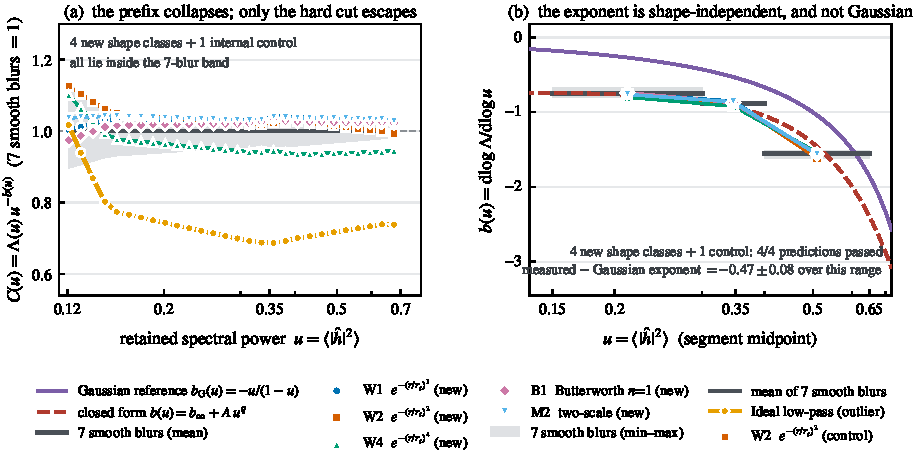
\includegraphics[width=\textwidth]{fig_law.pdf}
  \caption{%
    \textbf{(a)} The local normalisation $C(u)=\Lambda(u)\,u^{-b(u)}$ with $b(u)$ the exponent
    of panel~(b), normalised so that the geometric mean of the seven smooth blur kernels is $1$
    at each $u$; the shaded band is their min--max. This frozen-exponent diagnostic is distinct
    from the integrated shape factor $\mathcal M(\mathrm{shape})$ in Eq.~\eqref{eq:law}. It is
    used only to compare operators \emph{at fixed $u$}; it is not the integrated law itself.
    Four profile families that had not been measured before the test, plus a fifth kept as an
    internal control against the real library kernel (colour), stay near that band. The plotted
    original 20-image test has maximum excursion $1.0283$ and maximum mean-relative deviation
    $1.1270$; the 120-image re-evaluation gives $1.0425$ and $1.1257$, against the pre-registered
    excursion limit $1.10$. The ideal low-pass with a hard cut and no passband escapes.
    \textbf{(b)} The local exponent
    $b(u)=\mathrm{d}\log\Lambda/\mathrm{d}\log u$ measured on the three $u$ segments: the
    seven-kernel mean with its min--max band, the five new families, and the closed form
    $b(u)\approx-0.73-7.2\,u^{3.4}$. All five new families land on the same exponent.}
  \label{fig:law}
\end{figure*}

\paragraph*{Validation}
The law was validated out of sample before it was believed. Fitted on the eight reference
profiles, it was tested against four predictions written down in advance on five new operator
families---Weibull of orders $1$ and $4$, Butterworth of order $1$, a two-scale mixture, and a
synthetic zero-phase Gaussian included as a deliberate \emph{internal control}: it shares its
profile shape with a reference kernel but not its construction. All four predictions passed:
the exponent fell inside the old families' range in $14$ of $15$ segment-by-family cells---the
exception, W1's middle segment at $-0.79$ against a range of $[-0.91,-0.82]$, is outside by
$0.03$ and inside its own bootstrap standard error of $0.04$; every prefix landed within
$1.13\times$ of the old mean; and the control reproduced the real library kernel's $\mathcal M(\mathrm{shape})$ to a
median of $0.1\%$ ($0.999$). The out-of-sample content rests on the four new shape classes; the
fifth confirms the apparatus on a case whose answer is already known. This is the paper's most
durable quantitative claim, but it is a transport test of measured curves and their local
exponents/normalisation band. It is not a zero-measurement prediction of an arbitrary new
operator's $\Lam$ or $\mathcal M(\mathrm{shape})$, and it does not by itself establish an
improved deconvolution algorithm.

\paragraph*{Image bootstrap, coordinate sensitivity, and estimator dependence.}
A post-hoc image bootstrap (2000 replicates, seed 20261113, with the same resampled image
indices across all three families) gives three-family-mean 95\% intervals
$b_\infty\in[-0.7367,-0.7221]$, $A\in[-7.6602,-6.8310]$, and $q\in[3.3247,3.5231]$.
These intervals cover image sampling only. The first-20, first-60, and last-60 image fits give
$(b_\infty,A,q)=(-0.7129,-6.9380,3.2956)$, $(-0.7316,-7.2560,3.3959)$, and
$(-0.7276,-7.2032,3.4458)$, respectively. Repeating the same fit on the same stored $\Lam$
values but with $u_{\rm full}$ instead gives $(-0.7191,-7.1706,3.3881)$, with image-bootstrap
intervals $[-0.7259,-0.7116]$, $[-7.6008,-6.7827]$, and $[3.2930,3.4877]$. Per-family fit rms
changes by less than $0.001$, so the full-grid coordinate does not remove the empirical form.

The exact parameter vector is nevertheless estimator-dependent. Across degree 3--6 polynomial
derivatives and three closed-form windows ($[0.13,0.86]$, $[0.14,0.74]$, and $[0.18,0.65]$),
the family-mean ranges are $b_\infty\in[-0.8246,-0.4366]$, $A\in[-9.6622,-3.9867]$, and
$q\in[1.8514,4.0681]$. These are sensitivity ranges, not confidence intervals. The corresponding
ranges at measured coordinates are narrower: $b(0.35)\in[-1.0343,-0.8374]$ and
$b(0.65)\in[-2.4885,-2.2806]$. Changing the second-stage window leaves the polynomial derivative
unchanged but can alter the correlated extrapolated parameters substantially. We therefore claim
a useful negative, steepening exponent and a scoped empirical form, not a uniquely identified
$(b_\infty,A,q)$ independent of smoothing. Source: \texttt{results/review2\_statistics.json}.

\paragraph*{Shared-probe and integration-tolerance audit.}
We also repeated the complete 20-operator curve for W2/W8/TK50 on four fixed generated images
at $t=0.002$, using four independent Rademacher probes. Within each replicate the same probe is
shared by the sharp image and every $u$; probes differ across replicates. The three-family-mean
parameters have across-probe SD $0.00240$ ($b_\infty$), $0.0954$ ($A$), and $0.0317$ ($q$).
The maximum per-$u$ SD of $b(u)$ is $0.0287/0.0394/0.0467$ for W2/W8/TK50. With probe 0 held
fixed, changing RK45 rtol=atol from $10^{-5}$ to $10^{-6}$ changes $\Lam$ by at most
$4.33/4.11/5.27$ nats across the three families, and $b(u)$ by at most $0.0036/0.0117/0.0342$.
The corresponding largest absolute parameter changes over the three families are $0.00165$,
$0.0919$, and $0.0295$. These four-probe summaries are numerical-variability diagnostics on four
images, not precise confidence intervals or a solver guarantee for other models/noise levels.
Sources: \texttt{results/law\_stability.json} and
\texttt{results/law\_stability\_analysis.json}.

\paragraph*{The $t$-dependence, and what causes it.}
The closed form is the first candidate that survived internal consistency: fitted on a dense
$19$-point grid, three families of very different shape agree to within $0.345$ dex, far inside
the $0.50$ we had pre-registered, and four rival forms fit worse by $5$--$60\times$ or hit their
parameter bounds. The parameters quoted in \eqref{eq:law} are the three-family mean at
$t=0.002$; per family
$b_\infty\in[-0.743,-0.712]$, $A\in[-7.36,-7.11]$ and $q\in[3.33,3.49]$. Those parameters
nevertheless drift with $t$. Re-measured on $120$ images per operator, $b_\infty$ moves from
$-0.730$ to $-0.454$ over
$t\in[0.002,0.05]$, with the same sign in $12/12$ cases and beyond $2\,$SE in $12/12$; the
twenty-image scan had found $12/12$ and $10/12$, so the larger pool buys the two cells that were
borderline rather than changing the direction. The
\emph{form} keeps fitting at every $t$ in that range (rms $\le0.075$ against a $b$ that itself
spans $\sim4$; it degrades at $t=0.16$, see below). The drift is resolved in the reported 120-image fits; in the limited checkpoint comparison,
swapping EDM/FFHQ for EDM/AFHQv2 moves $b_\infty$ by $\le0.011$, a factor $25$ less than
the noise-level change. Its source is
measurable. Writing $\rho(t,u)=\Lam(t,u)/\Lam_0(u)$, the decay is close to linear,
$\rho\approx1-14\,t$ with $(1-\bar\rho)/t$ between $10.6$ and $16.1$, and $\rho$'s spread
between $u=0.85$ and $u=0.14$ grows monotonically from $6.7\%$ at $t=0.005$ to $78\%$ at
$t=0.05$---which is exactly the sequence $\Delta b_\infty=+0.036\to+0.276$. The mechanism is that $\Lam$ is a
small difference of two large numbers: at $t=0.002$ and $u=0.85$ it is $913$ nats against
$\Lambda_B=35752$ and $\Lambda_S=34839$, a $2.6\%$ sliver. The two large sides decay at nearly
the same rate---$0.9\%$ apart at $u=0.85$ over $t\in[0.002,0.05]$---yet $\Lam$ itself falls
$1.93\times$ faster than the mode they share at $u=0.85$, and the ratio grows as the blur
strengthens: $1.93\times$ at $u=0.85$, $2.12\times$ at $u=0.54$ and $2.32\times$ at $u=0.35$.
The cancellation is therefore not uniform in $u$, so an exponent measured at one $u$ does not
transport to another---which is the whole content of the $t$-dependence.

What we could \emph{not} do is close it. Four pre-registered parametrisations of the decay were
refuted. An earlier two-component Gaussian/non-Gaussian decomposition used the retired
unweighted-rFFT, channel-averaged reference, so its numerical drift predictions are not a valid
full-image Gaussian test and are withdrawn here. The full-FFT audit does not validate a
$t$-independent non-Gaussian exponent. The empirically observed $t$-dependence is therefore
traced through the unequal decay of the two large log-density terms above, but is not reduced
to a closed-form mixture; an estimator calibrated at one noise level need not transport to another.

\paragraph*{An asymptotic we had taken as clean, and lost.} On twenty images $b_\infty(0.16)$
read $+0.0023$, within noise of the Gaussian value $0$ of Eq.~\eqref{eq:lgauss}, and we had
reported convergence. On $120$ images it is $-0.211\pm0.026$---eight standard errors below zero,
and the three families agree in sign ($-0.281$, $-0.185$, $-0.167$). The exponent is still moving
toward $0$, from $-0.454$ at $t=0.05$, but at the highest noise level we measure it has not
arrived, and we do not claim convergence. The same run shows the closed form itself degrading
there: at $t=0.16$ one family's fit residual is $2.6\times$ its $t=0.002$ value, against
$\le1.7\times$ everywhere else. The Gaussian comparison has the different form
$b_{\rm G}(u_{\rm full})=-u_{\rm full}/(1-u_{\rm full})$; approaching it is a hypothesis about
the full-grid coordinate, not a formula we have established for the empirical $u$ curves.

\paragraph*{What sets $\mathcal M(\mathrm{shape})$?}
We could not find a single scalar descriptor for $\mathcal M(\mathrm{shape})$, and the negative results are themselves
informative. $B_2=\langle a^2\rangle/\langle a\rangle$ fits $R^2=0.825$ on seventeen profiles
but fails a pre-registered prediction test on five new shape classes ($1.61\times$ scatter at
matched $B_2$, non-monotone). A relative transition width $tw_{\rm lev}$ passes $5/6$ new
families and then fails decisively on the sixth. The refined descriptor
$tw_{\rm od}=tw_{\rm lev}/\text{dyn}$ predicts $\mathcal M(\mathrm{shape})$ to within $0.015$ dex for every operator
we measured that has a passband---a set that includes all the physical blur kernels we
measured---and degrades for the fourth class, where $g_2$ can reach $0$ but not $1$. The one descriptor that survives across classes is
the \emph{radial position of the transition band}: holding shape, $\langle a\rangle$ and
bandwidth fixed and moving the band from $r\approx0.66$ to $r\approx0.23$ moves $\mathcal M(\mathrm{shape})$ by a factor
$2.47$, where $tw_{\rm od}$ spans $2.11$ and the law predicts $1.08$. Our reading is that
$\mathcal M(\mathrm{shape})$ is \emph{regime-structured} rather than absent: which structural feature
matters depends on which regime the operator's spectrum occupies. Taken together, these descriptor
analyses are exploratory. They do not jointly identify transition position, roll-off rate,
anisotropy, spectral zeros, and passband support, and do not yield a unified predictor for an
unmeasured shape.

\paragraph*{A limited two-checkpoint comparison}
On the same EDM/AFHQv2-generated image pool, replacing EDM/FFHQ with EDM/AFHQv2 moves $\Lam$
by $0.7$--$3.5\%$ and $b_\infty$ by $\le0.011$ in our paired comparison. Holding the FFHQ
checkpoint fixed and changing the generated image pool moves $\Lam$ by $5.5$--$19.2\%$; the
two pools' outer-band spectra differ by $29\%$. The absolute prior-swap differences are
$7$--$1709$ nats (median $76$) over 60 paired operators; $59/60$ have one sign, although most
individual differences are below the $388$-nat pilot scale. For the exponent, $t$ moves
$b_\infty$ by $0.276$ versus at most $0.011$ under this checkpoint swap. This is evidence of
relative insensitivity \emph{between these two EDM checkpoints}, not prior-independence. The
binarized-MNIST reversal in \cite{nguyen2025morsebott} also shows that training distribution
can matter. Different architectures, noise parameterisations, and real-image domains remain
untested.

\section{Limits of stationary Gaussian and spectral approximations}
\label{sec:mech}

A local second-order Taylor approximation and a stationary Gaussian/spectral model are not the
same object. The former uses
$\log p_t(z)\approx\log p_t(x_0)+\nabla\log p_t(x_0)^\top(z-x_0)
+\tfrac12(z-x_0)^\top H_t(x_0)(z-x_0)$ with $H_t(x_0)=\nabla^2\log p_t(x_0)$, a generally
image-dependent and non-circulant Hessian. Our three references instead use a global covariance
or an operator power-spectrum functional, and are not equivalent to this local approximation.
We do not evaluate the full Hessian matrix; after the reference comparisons, we separately test
its restriction to one actual blur direction through the ODE potential.

\paragraph*{Reference 0: the isotropic Gaussian limit.}
For $p_t=\mathcal N(0,(s^2+t^2)I)$ and a fixed image, Parseval gives the exact expression
$\Lam_{\rm iso}(x,h)=(\|x\|^2-\|h\blur x\|^2)/(2(s^2+t^2))$; it is not generally a function of
the empirical $u$ alone. Averaging over an isotropic random image with per-coordinate second
moment $s^2$ gives, in the full-grid coordinate defined above,
\begin{equation}
  \begin{aligned}
  \bar\Lam_{\rm iso}(u_{\rm full}) &= (1-u_{\rm full})\,
  \frac{N s^2}{2(s^2+t^2)},\\
  b_{\rm G}(u_{\rm full}) &=-\frac{u_{\rm full}}{1-u_{\rm full}},
  \end{aligned}
  \label{eq:lgauss}
\end{equation}
because $\mathbb E\|h\blur x\|^2=u_{\rm full}Ns^2$. Here
$b_{\rm G}=\mathrm d\log\bar\Lam_{\rm iso}/\mathrm d\log u_{\rm full}$. Shape independence and
$b_{\rm G}(u_{\rm full})\to0$ as $u_{\rm full}\to0$ are statements about this isotropic average,
not an individual non-white image or the unweighted rFFT mean. The measured
$b_\infty\approx-0.73$ at $t=0.002$ differs from that limiting value; on 120 images
$b_\infty(0.16)=-0.21\pm0.03$, so the measured asymptote has not reached zero. We do not subtract
exponents evaluated at two different spectral-grid conventions. The earlier two-component drift
calculation based on the reduced reference is withdrawn rather than presented as a validated
mechanism.

\paragraph*{Reference 1: a spectral functional.}
For a zero-mean stationary Gaussian with shared covariance across independent RGB channels, let
$S(f)$ be the channel-averaged calibration spectrum and $\bar Z_x(f)$ the channel-averaged image
periodogram, both normalised by $HW$. The full real-image log-ratio is
\begin{equation}
  \Lam_G \;=\; \sum_{f\in\mathcal R}\big(1-g_2(f)\big)\,w_g(f),\qquad
  w_g(f)=\frac{3c_f\bar Z_x(f)}{2(S(f)+t^2)}.
  \label{eq:lamg}
\end{equation}
The factor three restores all RGB channels, and $c_f$ restores conjugate modes omitted from the
rFFT representation. For spatially decreasing spectra $w_g$ falls with radius. If the full-grid
weights are flat, $\Lam_G$ reduces to $\mathrm{cap}\,(1-u_{\rm full})$, as in Reference~0.

Over 851 operator rows from 19 sweep files, all using twenty generated images and spanning
$t\in[0.002,0.16]$, 61 empirical $u$ values and 42 operator families, the median of
$|\Lam_G/\Lam|$ is $1.002$ (95th percentile $4.570$, maximum $11.609$). At $t=0.002$ the median
is $0.789$; at $t=0.16$ it is $4.868$. Thus this reference captures a substantial share in the
median at low noise and often overestimates at high noise; the old claims of a $0.136$ median
share and a factor-30 shortfall are withdrawn. The discrepancy is strongly noise-level-dependent,
not a uniform failure of spectral modelling. For $t\to0$ and $\bar Z_x=S$, the corresponding
full-RGB ceiling is $3HW/2=6144$ nats. Two disjoint twenty-sample evaluations give $6215$ and
$6296$ nats, within $2.5\%$ of that value; the residual reflects their spectrum mismatch to the
256-sample calibration pool. Source: \texttt{results/fullfft\_reference\_audit.json}.

\paragraph*{Reference 2: a spectrum-matched Gaussian.}
This reference uses radially binned variances from calibration samples 0--127 plus $t^2$,
together with the sharp image's actual periodogram. It again includes $c_f$ and all three RGB
channels. It gives $2542.6$ nats at $t=0.002$, against the measured $31965.8$ nats, a
$12.57\times$ shortfall. At $t=0.10$ and $0.20$, however, it gives $1292.5$ and $725.0$ nats,
above the corresponding measured $916.5$ and $162.2$ nats. This plug-in Gaussian is therefore
inadequate at low noise in this example, not uniformly below the learned-prior preference.

\paragraph*{Sensitivity to the transition-band position.}
Holding the empirical attenuation coordinate fixed and moving only the \emph{radial position}
of the operator's transition band, the full-FFT $\Lam_G$ moves by $0.7$--$1.6\%$ while measured
$\Lam$ moves by $40$--$227\%$ and changes sign; the paired difference is significant at
$9$--$22\sigma$ under the reported image bootstrap. Thus this particular spectral functional is
comparatively insensitive to a feature that strongly affects the measured preference. This
controlled result does not imply that every covariance-based or local-Hessian approximation must
behave likewise.

\paragraph*{A directional local-quadratic check of the ODE potential.}
To test a genuine local second-order object rather than a denoiser Jacobian, let
$\delta=h\blur x-x$ and evaluate the ODE potential $q_t(x+s\delta)$ along the actual blur line.
The directional gradient and Hessian curvature are estimated from $s=\pm0.5$; their quadratic
prediction of $q_t(x+\delta)-q_t(x)$ is compared with the independently evaluated $s=1$ point.
All points within a line share one Rademacher vector. For the generated image used above and
Gaussian $\sigma=1.5$, the actual change at $t=0.002$ is $-32048.7$ nats, whereas the prediction
is $-15225.7$ (absolute error $16823.1$). For a real BSDS image, the corresponding values are
$-37199.7$ and $-15383.5$ (error $21816.2$). At $t=0.20$, the actual/predicted changes are
$-206.1/-28.35$ (error $177.75$) and $-1613.4/-1987.8$ (error $374.40$), respectively. The
alternative fit from $s=\pm0.25$ gives larger errors: $19802.2$ and $24476.3$ at low noise,
and $304.37$ and $546.51$ at high noise, in the same generated/real order. Thus reducing the
fit spacing does not rescue the extrapolation to $s=1$ in these cases. Sharing one trace vector
removes independent Hutchinson jitter along each line, but two spacings cannot separate all
finite-difference, ODE, and genuine nonlinear contributions. The test covers only one direction
per image/noise setting and is not a full-Hessian or all-local-methods failure theorem. Source:
\texttt{results/local\_quadratic\_analysis.json}.

\paragraph*{Accurate moments do not validate a Gaussian inference formula.}
The variance of the data term follows its second-order prediction: over
$\sigma_n\in[0.02,0.1]$ its median falls by $627\times$ against a predicted $625\times$
($1.003\times$), and collapse points agree to three digits across all $51$ operators on a
$\sigma_n$ grid spanning $15000\times$. By contrast, substituting a measured variance into a
Gaussian formula for the effective sample size of prior importance sampling is wrong by
$6.7\times10^{13}$ at $\sigma_n=12$, by $1.1\times10^{5}$ at $\sigma_n=15$, and by
$19$--$26\times$ at $\sigma_n=20$. This isolates the error in the tested Gaussian mapping,
not in the arithmetic used to estimate the variance.

\paragraph*{Scope for algorithms.}
The results show reference- and noise-level-dependent Gaussian/spectral errors, and identify a
specific missing structural sensitivity. They do not show that all stationary approximations
underestimate $\Lam$, that all second-order algorithms fail, or that no scalar diagnostic can
work outside the tested regime.

\section{Objective, optimisation map, and an algebraic no-blur gap}
\label{sec:map}

We first delimit the statistical model. For observation noise level $\sigma_n$, let
\begin{equation}
  \begin{aligned}
  D_\theta(x;y)&=\frac{\|h_\theta\blur x-y\|^2}{2\sigma_n^2},\\
  L(x,\theta;y)&=D_\theta(x;y)+q_t(x),
  \end{aligned}
  \label{eq:map_objective}
\end{equation}
where $q_t=-\log p_t$ is always the prior potential and $D$ is always the data-fidelity term.
The profile-MAP objective, rather than a profile likelihood because it contains a prior, is
\begin{equation}
  \ell_y^{\rm opt}(\theta)=\min_x L(x,\theta;y).
  \label{eq:profile}
\end{equation}
If a latent image $z$ is generated from $p_t$ and $y=h_\theta\blur z+\eta$, then
\eqref{eq:map_objective} is its joint negative log-posterior up to constants and any operator
prior. If instead $x_0\sim p_0$ and $y=h_\theta\blur x_0+\eta$, its exact clean-image prior is
$q_0$, not $q_t$. Setting $t=\sigma_n$ does not by itself make the smoothed density $p_t$ the
correct prior for that clean-image posterior. Our experiments therefore concern the explicitly
declared \emph{smoothed-prior MAP surrogate} \eqref{eq:map_objective}, not an exact posterior
for the original $p_0$ generative process.

For $y=h_{\theta^\blur}\blur x^\star+\eta$, define the generating-pair values
$D_\star=\|\eta\|^2/(2\sigma_n^2)$ and
$L_\star=L(x^\star,\theta^\blur;y)=D_\star+q_t(x^\star)$. The data term does not vanish when
observation noise is present.

\paragraph*{The denoiser is not generally the proximal map of $q_t$.}
For an ideal MMSE denoiser $D_t$, Tweedie's identity gives
\begin{equation}
  \nabla q_t(v)=\frac{v-D_t(v)}{t^2},\qquad
  D_t(v)=v-t^2\nabla q_t(v).
  \label{eq:tweedie_gradient}
\end{equation}
By contrast, $z=\operatorname{prox}_{q_t/\rho}(v)$ requires the implicit condition
$z+\rho^{-1}\nabla q_t(z)=v$. The denoiser evaluates the gradient at $v$ and is not generally
that implicit solution. It can motivate a plug-and-play prior update, but this does not
establish that the resulting fixed point minimises $L$.

Our implemented iteration is Douglas--Rachford-type, not the originally assumed HQS update. With
$d^k=D_{\sigma_n}(z^k)$, $v^k=2d^k-z^k$, $K_\theta=\mathcal Fh_\theta$, and $\sigma_n=t$,
the complete update is
\begin{align}
  x^{k+1}&=\mathcal F^{-1}\!\left[
  \frac{\overline{K_\theta}\,\hat y+\hat v^k}{|K_\theta|^2+1}\right],\nonumber\\
  z^{k+1}&=\Pi_{[-1,1]}(z^k+x^{k+1}-d^k),\qquad \hat x_{\rm PnP}=D_t(z^K).
  \label{eq:pnp_updates}
\end{align}
The Fourier data step is exact, but the denoiser substitution has no proximal-map or
local-minimum guarantee for $q_t$. Accordingly, we call the subsequent grid selections
\emph{PnP-profile minima}, not minimisers of $\ell_y^{\rm opt}$. Section~\ref{sec:overblur}
therefore also tests the latter with direct score-gradient optimisation, while retaining its
approximate, non-global status.

\paragraph*{An identity that remains valid without convergence.}
Let $\hat x_0$ be the PnP output at $\theta=0$, and define
$D_{\rm PnP}=D_0(\hat x_0;y)$ and $E_{\rm PnP}=L(\hat x_0,0;y)-L_\star$. With
$x^\blur=h_{\theta^\blur}\blur x^\star$ and
\begin{align}
  \Delta q_t&:=q_t(\hat x_0)-q_t(x^\blur),\\
  \Lam_{\rm clean}(t)&:=q_t(x^\star)-q_t(x^\blur)
  =\log p_t(x^\blur)-\log p_t(x^\star),
  \label{eq:identity_defs}
\end{align}
direct substitution gives
\begin{align}
  E_{\rm PnP}
  &=D_{\rm PnP}+q_t(\hat x_0)-D_\star-q_t(x^\star)\nonumber\\
  &=\Delta q_t-\Lam_{\rm clean}(t)+(D_{\rm PnP}-D_\star).
  \label{eq:identity}
\end{align}
Here ``clean'' describes the noise-free input pair, not $t=0$. Equation~\eqref{eq:identity}
is pure algebra and holds for any $\hat x_0$ and any prior. If the inner minimum is solved
exactly, the same calculation applies to $E_0=\ell_y^{\rm opt}(0)-L_\star$.

The identity's limited use is to separate the clean-pair preference from the image-update prior
change and the data-fit change. A computed $E_{\rm PnP}<0$ supplies a feasible no-blur point
with lower surrogate objective than the generating pair, and therefore certifies that the
latter is not a global minimiser of this surrogate. A nonnegative PnP value is inconclusive.
Moreover, $\Delta q_t$ and $D_{\rm PnP}$ depend on the PnP output; the identity does not predict
the gap without optimisation. Its numerical residual, at most $1.6\times10^{-14}$ in the
reported 75-configuration check, verifies floating-point bookkeeping only, not a new MAP
theorem. The separate 20-image run gives the same algebraic check by construction.

Neither $\Delta q_t$ nor $D_{\rm PnP}$ is prior-independent. FFHQ/AFHQv2 per-strength ratios
differ by $0.004$--$0.033$ in our experiments, within the reported combined $2\,$SE, but this is
a limited numerical comparison and not a proof of prior independence. Cross-strength
universality of a single $\Lam_{\rm clean}$-only predictor is rejected ($\|t\|=10.6$); the two
additional terms cannot be discarded.

\paragraph*{Sample-wise sign consistency, not a universal lemma test.}
Lemma~12 of \cite{nguyen2025morsebott} requires $q(h\blur x)\le q(x)$ for all $x$ and all $h$
in its kernel set. For one fixed pair at fixed $t$, this is exactly
$\Lam_{\rm clean}(t)\ge0$ by~\eqref{eq:identity_defs}. In 15 pilot configurations, the
predicted relationship held in $15/15$ cases: $\Lam_{\rm clean}>0$ corresponded to
$E_{\rm PnP}<0$, while the single $\Lam_{\rm clean}<0$ case had $E_{\rm PnP}>0$. This is an
empirical sign-consistency observation for those pairs. It does not establish the universally
quantified hypothesis, decide the lemma's validity boundary, or prove convergence to a profile
minimum.

\paragraph*{Relation to known MAP instability.}
Buskulic and Calatroni \cite{buskulic2026maplmmse} study synthetic blind deconvolution with
complete signal and kernel distributions and report MAP instability alongside a more robust
LMMSE estimator. That work concerns a different, fully specified statistical setting. Our
identity is complementary bookkeeping for a learned-prior objective; it is not a sharper
stability theorem or a restoration algorithm.

\section{Plug-and-play numerical profiles are setting-dependent}
\label{sec:overblur}

We first test where the PnP-generated grid's lowest measured surrogate objective lies, and then
probe new strengths and kernel families. This is not a profile-MAP convergence result: the
iteration in~\eqref{eq:pnp_updates} need not minimise the inner problem. Nor is positive
$\Lam$ on a fixed clean pair sufficient to predict a noisy-operator estimate. Term
decompositions describe selected grid points; they do not prove causality or universality.

\paragraph*{Optimisation protocol.}
The observation is $y=h_{1.5}\blur x^\star+\eta$ for a symmetric $15\times15$ Gaussian kernel
and each of the first twenty EDM/FFHQ-generated samples (pool indices 0--19). The operator grid
contains 21 strengths, $\theta\in\{0,0.125,\ldots,2.5\}$. At each grid point, the image
subproblem uses 240 iterations of the PnP--Douglas--Rachford update in~\eqref{eq:pnp_updates},
with the EDM denoiser evaluated at $\sigma_n$ and clipping to $[-1,1]$. Two initialisations,
$y$ and $h_\theta\blur y$, are run and the lower final $L=D+q_{\sigma_n}$ is retained. The
numerical PnP profile is the minimum of these two runs at each $\theta$, and
$\theta_{\rm grid}$ is the lowest of its 21 grid values. This is a feasible-point comparison,
not a certified inner minimum or a global profile minimum. A separate pilot diagnostic varied
60/240/600 iterations and three initialisations (including a random start), observing
$0.3$--$1.5\%$ variation across iteration counts and $1$--$3\%$ across starts; this does not
establish convergence or eliminate cross-grid Hutchinson variability. All grid points use the
same protocol to avoid changing the optimisation budget with $\theta$. Source:
\texttt{repro/repro\_phaseC\_pool20.py}.

\paragraph*{PnP-grid result with image-level dependence accounted for.}
At the four high noise levels $\sigma_n\in\{0.172,0.2455,0.3504,0.5\}$, $\theta_{\rm grid}$
exceeds $\theta^\blur=1.5$ in $79/80$ configurations; the exception equals the true strength.
The mean factor $\theta_{\rm grid}/\theta^\blur$ is $1.5323$ (observed range
$1.000$--$1.667$). These counts are not estimates of the $79/80$ proportion for exact
profile-MAP minimisers. The four configurations from one image are not independent. A post-hoc
percentile bootstrap that resamples all four configurations as a whole-image cluster (100,000
repeats, seed 20261109) gives 95\% intervals $[0.9625,1]$ for the over-blur proportion and
$[1.4938,1.5656]$ for the mean factor. These intervals quantify variability over the twenty
generated images, not across kernel families, model architectures, or real-image populations.
The fixed observation-noise seed schedule is reused at corresponding indices and noise levels
in the two pools, so these are not independent noise-replication intervals. Source:
\texttt{results/overblur\_cluster.json}.

Across the $400$ high-noise (configuration, grid-point) pairs with $\theta\in[2.0,2.5]$, the
advantage over $\theta^\blur$ ranges from $-2713$ to $4804$ nats and $393$ ($98.2\%$) favour an
over-blurred operator. Seven do not, and even the best single interval point fails in one
configuration ($-1591$ nats). Thus the result is distributional, not a per-image guarantee. A
separate two-image pilot comparing the corrected and half-pixel-shifted kernels changes the mean
factor by only $0.010$; this limited control does not establish invariance to other kernel sizes,
shapes, or directions.

\paragraph*{New strengths and kernel families overturn a universal reading.}
We next used eight previously unused samples from the same generated pool (indices 40--47),
noise levels $0.172$ and $0.5$, and the same 240-iteration/two-start protocol.
Table~\ref{tab:overblur_generalization} gives the full outcome. Only $19/64$ configurations
over-blur, whereas $37/64$ under-blur. At $\sigma_n=0.172$, $19/32$ over-blur; at
$\sigma_n=0.5$, none over-blur and $30/32$ under-blur (mean factor $0.646$, whole-image cluster
95\% interval $[0.566,0.717]$). The original $79/80$ result therefore cannot be extrapolated
across kernels, strengths, or noise levels. The eight-sample pilot is likewise not proof of
universal under-blurring; it demonstrates setting dependence.

\begin{table}[t]
  \centering
  \caption{Multi-kernel PnP-profile pilot on eight further EDM/FFHQ-generated samples and two
  noise levels. ``Over'' and ``Under'' compare the lowest measured PnP-grid point with the true
  grid value; they are not certified profile-MAP argmins. The Gaussian $\theta^\star=2$ arm
  initially omitted 2.0 from its grid; we evaluated that missing point with the frozen protocol
  after inspecting the initial profiles and use the completed PnP grid throughout. Source:
  \texttt{results/overblur\_generalization\_analysis.json}.}
  \label{tab:overblur_generalization}
  \small
  \setlength{\tabcolsep}{4pt}
  \begin{tabular}{lcccc}
    \toprule
    Family / $\theta^\star$ & Over & Under & Factor & Abs.\ error \\
    \midrule
    Gaussian / 1.0 & $7/16$ & $7/16$ & 1.081 & 0.294 \\
    Gaussian / 2.0 & $3/16$ & $10/16$ & 0.762 & 0.301 \\
    Defocus / 1.5 & $7/16$ & $8/16$ & 0.975 & 0.313 \\
    Motion / 3.0 & $2/16$ & $12/16$ & 0.604 & 0.427 \\
    \midrule
    Pooled & $19/64$ & $37/64$ & 0.856 & 0.334 \\
    \bottomrule
  \end{tabular}
\end{table}

\begin{figure*}[t]
  \centering
  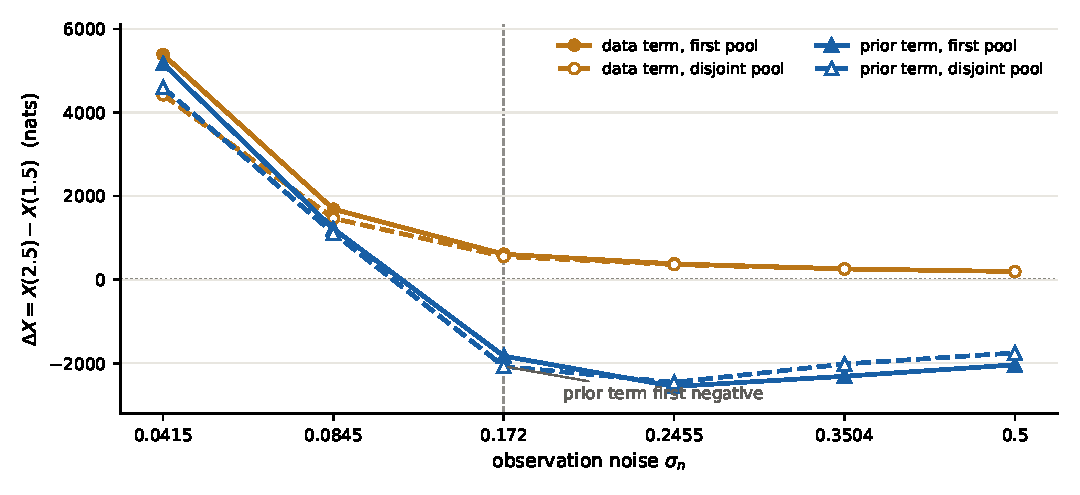
\includegraphics[width=\textwidth]{fig_overblur_terms.pdf}
  \caption{%
    Two-term comparison at the fixed grid points $\theta=1.5$ and $2.5$, with
    $\Delta X=X(2.5)-X(1.5)$ averaged over generated images. Solid: pool indices 0--19;
    dashed: the disjoint index set 20--39 from the same EDM/FFHQ-generated pool, measured
    against criteria fixed before collection. The data term (circles) decays with observation
    noise; the prior term (triangles) changes sign between $\sigma_n=0.0845$ and $0.172$ and
    saturates near $-2\times10^3$~nats. This fixed-grid association is not a decomposition at
    a certified profile-MAP optimum or evidence that the PnP inner iteration minimises $L$.}
  \label{fig:overblur_terms}
\end{figure*}

\paragraph*{Associated objective-term changes at fixed grid points.}
Each stored PnP profile separates $L=D+q$. Figure~\ref{fig:overblur_terms} shows
$\Delta D$ falling from $+5388$ to $+193$~nats as $\sigma_n$ goes from $0.0415$ to $0.5$,
following $\sigma_n^{-1.35}$ ($R^2=0.99$); the second-pool exponent is $1.27$. Over the
same range $\Delta q$ changes from $+5170$ to about $-2\times10^3$~nats. Hence, at these two
fixed grid points, the prior difference increasingly favours $\theta=2.5$ as noise grows.

Four decisive criteria fixed before the second-pool measurement passed. In a data-term-only
ablation, $0/120$ second-pool configurations over-blur ($2/120$ on the first pool), which
shows that the prior term is required for the observed PnP-grid shift under this protocol. The
fixed-point $\Delta q$ first turns negative at $\sigma_n=0.172$ on both pools, and the
second-pool decay exponent $1.273$ lies in its pre-registered interval $[1.250,1.459]$.

We also decomposed the selected PnP-grid point, rather than only the fixed endpoints. Relative
to the true-strength grid point, the main pool gives mean $\Delta D=+225.9$ and
$\Delta q=-2346.1$ nats; the disjoint second pool gives $+251.6$ and $-2181.3$ nats,
respectively. Whole-image cluster 95\% intervals are $[185.5,269.2]$ and $[-2550.6,-2138.4]$
on the main pool, and $[217.9,288.4]$ and $[-2422.4,-1936.6]$ on the second pool.
The prior change is negative in $79/80$ and $80/80$ high-noise configurations. A negative total
$\Delta L$ is tautological after selecting the lowest measured grid point; these term magnitudes
do not alone prove causality or profile-MAP convergence. Source:
\texttt{results/overblur\_optimum.json}.

\paragraph*{A fixed spectral correction does not consistently improve kernel error.}
We tested $L_{\rm corr}(\theta)=L(\theta)+\Lambda_G(\theta,t)$ on the stored PnP outputs with
coefficient fixed at one, where
$\Lambda_G=3\sum_{f\in\mathcal R}c_f(1-g_{2,\theta})S/(2(S+t^2))$ and $S$ is the
channel-averaged spectrum of the separate calibration samples 128--255. This is the full-RGB,
conjugate-complete stationary spectral-Gaussian component, with no test-image fitting or tuning
against the outcome. It changes $3/80$ PnP-grid minima on each pool. Over-blurring changes from
$79/80$ to $78/80$ on the main pool and remains $80/80$ on the second. Mean absolute relative
kernel error changes from $0.5323$ to $0.5365$ on the main pool, but from $0.5615$ to $0.5531$
on the second. Post-hoc image-cluster 95\% intervals for the error difference are
$[-0.0042,0.0188]$ and $[-0.0177,0]$, respectively. Thus there is no consistent improvement to
justify downstream restoration claims. The retired reduced-grid correction left every PnP-grid
minimum unchanged and is kept only as an audit trail. Source:
\texttt{results/blur\_correction\_fullfft.json}.

\paragraph*{Real-image PnP-profile pilot.}
We repeated the same 21-point Gaussian $\theta^\star=1.5$ grid and 240-iteration/two-start
PnP--Douglas--Rachford protocol on the first eight real BSDS test images at
$\sigma_n\in\{0.172,0.5\}$. Only $4/16$ PnP-grid minima over-blur and $12/16$ under-blur (mean
factor $0.6198$, mean absolute relative kernel error $0.5156$). At $\sigma_n=0.172$, $4/8$
over-blur and $4/8$ under-blur; at $\sigma_n=0.5$, all $8/8$ under-blur. Relative to the
true-strength grid point, the mean changes are $\Delta D=-100.1$ and $\Delta q=-42.1$ nats, a
descriptive decomposition rather than a causal proof. The real profiles are especially flat:
top-five spreads are $9.65$--$586.1$ nats, so many grid differences are below or comparable to
the $388$-nat pilot scale. This real-data pilot reinforces setting dependence but is too small
and numerically flat to support universal under-blurring. Sources:
\texttt{results/real\_bsds\_profile.json} and \texttt{results/real\_profile\_analysis.json}.

\paragraph*{Direct score-gradient consistency pilot.}
To test the declared objective rather than the PnP fixed point, we implemented the actual
first-order gradient
$\nabla_xL=A_\theta^\top(A_\theta x-y)/\sigma_n^2+(x-D_{\sigma_n}(x))/\sigma_n^2$.
At each of the same 21 Gaussian strengths, Adam runs for 600 steps from $y$ and
$h_\theta\blur y$ (initial learning rate $0.003$, cosine decay to $5\%$), without clipping
because~\eqref{eq:map_objective} is unconstrained. The lower final $L$ is selected per grid point.
Initial and final $q$ are evaluated by the ODE with one Rademacher vector shared across each
profile. Two generated images and two real BSDS images are each tested at
$\sigma_n\in\{0.172,0.5\}$. This pre-registered protocol is a small consistency pilot, not a
replacement population estimate.

All $336/336$ generated-plus-real runs decrease their measured final $L$ relative to their
initialisation. The score-grid selections under-blur in $4/4$ generated and $4/4$ real
configurations, with mean $\theta_{\rm grid}/\theta^\star=0.1458$ and $0.125$, respectively.
On the same generated configurations, PnP instead over-blurs $4/4$. The selected score-grid
point is $1750$--$2931$ nats below the true-strength point across these eight profiles. The
largest directional score/ODE relative discrepancy at the tested $\theta=0$ endpoint is
$3.97\%$ on generated and $5.62\%$ on real images. These checks establish a substantially
closer connection to the declared gradient, not global optimality. The maximum final gradient
RMS across all runs is $12.50$; at selected points it is $0.876$--$3.132$, and their last-50-step
RMS drift is $4.9\times10^{-4}$--$2.35\times10^{-3}$. Unconstrained iterates can exceed the
training pixel range (maximum $|x|=2.064$), so this experiment is not a restored-image quality
claim. Sources: \texttt{results/score\_profile\_generated.json},
\texttt{results/score\_profile\_real.json}, and
\texttt{results/score\_profile\_analysis.json}.

\paragraph*{Endpoint trace replication.}
Without reoptimising, we re-evaluated all $336$ stored final images with four probes per
profile: the reconstructed original probe and three independent probes, each shared across all
42 endpoints of that profile. A separate batch-size-one check reproduces the original stored
$q$ to within $0.0234$ nats, while the batched recheck differs from that B1 value by at most
$1.43$ nats. All $32/32$ probe-specific grid selections and all $8/8$ four-probe-mean profiles
under-blur. The maximum endpoint $q$ SD across four probes is $64.8$ nats. The mean-profile
selection remains $1756$--$2944$ nats below the true-strength point, with mean-profile top-five
spreads of $321$--$1090$ nats. At $\sigma_n=0.172$, the probe-specific minima move only within
$0$--$0.25$ (generated) and $0$--$0.125$ (real), so their exact low-blur rank is not resolved.
At $\sigma_n=0.5$, every probe selects $0.375$ in all four profiles. These replicates separate
trace variability from optimisation error; they do not turn four probes into a confidence
interval or establish a global minimum. Sources:
\texttt{results/score\_profile\_generated\_recheck.json},
\texttt{results/score\_profile\_real\_recheck.json}, and
\texttt{results/score\_profile\_probe\_b1.json}.

\paragraph*{Grid-selection resolution.}
The spread of the PnP profile over its five best grid points is $136$--$6341$ nats across
all 120 profiles ($136$--$3695$ nats across the 80 high-noise ones). The lower values are below
or comparable to the $388$-nat Hutchinson pilot scale, so some grid selections are resolvable
only to approximately one grid step; the larger spans show that this limitation is not uniform.
This grid-resolution statement is distinct from the missing inner-minimum guarantee.

\section{A kernel bug, and what it did and did not corrupt}
\label{sec:bug}

We report this because it changed numbers in the paper and because the way it was caught is the
paper's methodological lesson.

Thirteen of our scripts constructed the Gaussian kernel on a hand-written coordinate grid
(three further scripts carry that grid as the faulty arm of a comparison, and
are not counted here)
\begin{equation}
  \texttt{-(ks//2)+1} \;=\; \texttt{-6},
\end{equation}
whereas the library's \texttt{-ks//2+1} evaluates to $(-ks)//2+1=\texttt{-7}$, because Python's
unary minus binds more tightly than floor division. The resulting kernel was
\textbf{asymmetric}, with its peak shifted one pixel and
$\max|k-\mathrm{flip}(k)|=3.159\times10^{-2}$. It was not the intended centred, symmetric
Gaussian blur.

\paragraph*{How it was caught.}
Re-running a published result with the same seed and the same script reproduced every digit,
including a single anomalous cell. Only a cross-implementation check---the same physics with
the kernel taken from the library instead of hand-written---failed. \emph{Shared bugs are
invisible to same-seed reproduction.} This is why the current Gaussian, defocus, Airy, and
motion kernels come from the library; the ideal low-pass and synthetic spectral gates are
constructed explicitly as described in Section~\ref{sec:law}.

\paragraph*{Blast radius.}
The corrected $\Lam(t)$ table is Table~\ref{tab:lamt}: the error raised $\Lam$ by
$2.4$--$8.0\%$ at $t\le0.02$ (e.g.\ $33898\to31966$ at $t=0.002$); changes at $t\ge0.05$ are
below the four-repeat pilot scale. The corrected $t=0.002$ value $31965.8$ agrees with a
separately produced twelve-image mean of $32081.0$ to $0.36\%$, whereas the uncorrected value
was off by $4.3\%$.

Beyond that table the bug shifted $\Lam_{\rm clean}$ by $4.0$--$8.5\%$ (mean $-389$ nats over
120 cells), without changing the reported sign and ordering outcomes. The mean ratio reproduced
to $0.0002$ ($1.1057\pm0.0125$ before, $1.1055\pm0.0080$ after), and the two-image cross-kernel
over-blur factor moved by $0.010$. On 252 overlapping measurements the absolute shift was $+649$
nats, comparable to the pilot Hutchinson scale. Quantities used here were re-measured with the
corrected kernel, including the twenty-image over-blur study. The threshold-dependent MAP check
changed from 76 to 75 configurations and from a $14.6\times$ to a $12.9\times$ span. The
algebraic identity is unaffected by construction. The two-checkpoint ratio comparison also
remains within its combined $2\,$SE, with raw differences of $0.004$--$0.033$; this is not
described as prior-independence.

\section{Limitations}
\label{sec:limits}

\begin{enumerate}
  \item \textbf{Models, input distribution, and resolution.} The main evidence is EDM/FFHQ at
        $64\times64$, with EDM/AFHQv2 as a second-checkpoint comparison and generated main pools.
        Real BSDS300 supplies a selected 32-image density test and eight-image PnP-profile pilot.
        The ADM arms use a continuous VP-ODE surrogate, not the original discrete models' exact
        normalised densities. The conditional 128 arm cannot isolate resolution from architecture,
        training data, or conditioning. Real FFHQ, a genuinely continuous-time non-EDM score model,
        unconditional high-resolution models, and broad natural-image universality remain untested.
  \item \textbf{Kernel scope.} The main two-pool PnP-grid result remains specific to a
        $15\times15$ Gaussian kernel at true strength $1.5$. The eight-sample pilot adds
        Gaussian strengths 1 and 2, Defocus 1.5, and Motion 3, and finds frequent under-blurring
        rather than reproducing the main proportion. Non-uniform blur, other kernel sizes, and a
        larger joint kernel/strength design remain untested.
  \item \textbf{Numerical density estimation and fitted-parameter uncertainty.} The 32-repeat
        Hutchinson study covers one image/operator at two noise levels. The new shared-probe
        audit propagates four independent traces through all 20 operators and the nonlinear fit,
        but only for four images, three families, and $t=0.002$. Its strict-tolerance arm is
        RK45, not a full-curve DOP853 comparison; DOP853 remains limited to the reported points.
        Image bootstrap, probe variability, solver tolerance, and polynomial/window sensitivity
        are reported separately rather than combined into a claimed total confidence interval.
        ADM precision checks are limited to the reported points. The exact terminal contribution
        is measured on 960 pairs and bounded in Eq.~\eqref{eq:terminal_bound}.
  \item \textbf{Plug-and-play is not profile-MAP convergence.} The denoiser is not generally
        $\operatorname{prox}_{q_t/\rho}$. The PnP--Douglas--Rachford iteration uses a fixed
        budget and two starts, need not attain even a local inner minimum of $L$, and its
        stochastic density estimates can affect grid comparisons. Its $79/80$ PnP-grid count is
        not a $79/80$ exact profile-MAP result. The direct score-gradient arm tests only two
        generated and two real images at two noise levels. Its 600-step endpoints still have
        nonzero gradients and no global certificate; four-probe replication measures endpoint
        density variability, not optimisation convergence. The $t=\sigma_n$ objective remains
        a smoothed-prior surrogate, and cluster intervals do not include optimisation, model,
        or kernel uncertainty.
  \item \textbf{No general second-order or MAP theorem.} Section~\ref{sec:mech} tests stationary
        Gaussian/spectral references and one actual blur direction per image/noise setting, not
        multiple directions or the full Hessian. Two finite-difference spacings do not separate
        every source of local approximation error. Equation~\eqref{eq:law} is an empirical fit
        whose parameters drift with $t$ and whose shape factor lacks a unified descriptor.
        Equation~\eqref{eq:identity} is algebraic; it neither proves a universal Lemma~12
        hypothesis nor predicts a profile gap without an inner solution. Fixed-grid and selected-
        point decompositions do not identify causal effects.
  \item \textbf{Sample sizes and dependence.} The main law and Fig.~\ref{fig:phen} use 120
        generated images per operator; the shared-probe curve audit uses four. The two 20-image
        PnP pools are disjoint index sets from one generated pool, not independent real-data
        cohorts. The multi-kernel pilot uses eight samples. The real density test uses the first
        32 sorted BSDS images, its PnP pilot eight, and the directional Taylor test one generated
        and one real image. The direct score pilot uses two generated and two real images at two
        noise levels. Raw image--kernel pairs within one image are dependent; exact sign intervals
        use the image as the independent unit and do not imply universal population probabilities.
  \item \textbf{No demonstrated restoration improvement.} The full-FFT $\Lambda_G$ correction
        changes some PnP-grid minima, but mean kernel error worsens on the main pool and improves
        only slightly on the second. We do not compare against LADiBI \cite{bai2026ladibi};
        without a consistent kernel-estimation improvement, we did not run downstream PSNR/SSIM
        experiments. The paper supports diagnostics and further correction research, not an
        improved restoration algorithm.
\end{enumerate}

\section{Conclusion}
\label{sec:concl}

For the tested EDM checkpoints and their generated $64\times64$ image pools, paired
probability-flow ODE measurements reveal a large clean-image blur preference and an empirical,
noise-level-dependent spectral scaling law. The preference holds in all 256 low-noise pairs on
32 selected real BSDS images, corresponding to $32/32$ image-level successes and exact 95\%
interval $[0.8911,1]$. At $t=0.20$, $120/128$ raw pairs are positive, while $27/32$ images are
positive on all four tested kernels. The ADM surrogate pilots establish model/noise dependence
only within those constructed priors. The fitted law now has image-bootstrap intervals, a
full-FFT-coordinate refit, shared-probe full-curve variability, and explicit polynomial/window
sensitivity; its precise parameters are not estimator-independent. Full-Fourier, full-RGB
references expose a $12.57\times$ low-noise shortfall in one example and strongly noise-dependent
errors across the wider audit. The directional Taylor test remains limited to one direction per
image/noise setting. In blind deconvolution, PnP-grid selections are not certified profile-MAP
minima. The direct score-gradient pilot instead under-blurs in all $32/32$ probe-specific and
$8/8$ four-probe-mean profiles, while still lacking a global-optimality certificate and precise
low-noise argmin resolution. This contrast demonstrates an algorithm-interpretation boundary,
not a universal operator-estimation rule or restoration improvement. Clean-pair preference is
not noisy-posterior preference. Broader real-image validation, larger direct optimisations
across kernels/models, joint uncertainty propagation in broader settings, and public archiving
remain necessary.

\section*{Data and Code Availability}

The reproducibility package comprises sweep scripts, criteria recorded before the
corresponding runs, offline judges, raw JSON results, figure scripts, and the image-pool
provenance described in Section~\ref{sec:pools}. It includes the full-FFT audit, ADM VP-ODE
adapter, direct score optimiser, saved endpoint images, verbatim Rademacher probes, endpoint
replications, and official checkpoint source/hash manifests; retired reduced-grid outputs remain
unchanged for auditability. Scripts retain their criteria and self-reported preregistration dates;
post-hoc analyses are labelled separately. These self-reports are not independent timestamp
certification. The public repository is
\url{https://github.com/BinNong/diffusion-blur-preference}; the immutable release is
\url{https://github.com/BinNong/diffusion-blur-preference/releases/tag/v1.0.1}, archived at
Zenodo under \url{https://doi.org/10.5281/zenodo.24279314}. The SHA-256 manifest includes
official source, environment versions, EDM/ADM checkpoint hashes, image indices, raw results,
and execution commands, but no model weights or credentials. Executable guards in
\texttt{repro/validate\_review2\_physics.py} check all eight reference kernels and 69 raw
synthetic-operator rows for symmetry/normalisation, conjugate-complete coordinates, and Parseval
consistency.

\bibliographystyle{IEEEtran}
\bibliography{refs}

\end{document}
